\documentclass[10pt,landscape]{article}
\usepackage{multicol}
\usepackage{calc}
\usepackage{ifthen}
\usepackage[a4paper, landscape]{geometry}
\usepackage{hyperref}

\usepackage{graphicx}
\graphicspath{ {./images/} }

\usepackage{listings}
\lstset{
    basicstyle=\ttfamily,
    breaklines=true,
    prebreak = \raisebox{0ex}[0ex][0ex]{\ensuremath{\hookleftarrow}},
    tabsize=2,
    gobble=8,
    frame=single
}

% This sets page margins to .5 inch if using letter paper, and to 1cm
% if using A4 paper. (This probably isn't strictly necessary.)
% If using another size paper, use default 1cm margins.
\ifthenelse{\lengthtest { \paperwidth = 11in}}
{ \geometry{top=.5in,left=.5in,right=.5in,bottom=.5in} }
{\ifthenelse{ \lengthtest{ \paperwidth = 297mm}}
{\geometry{top=1cm,left=1cm,right=1cm,bottom=1cm} }
{\geometry{top=1cm,left=1cm,right=1cm,bottom=1cm} }
}

% Turn off header and footer
\pagestyle{empty}


% Redefine section commands to use less space
\makeatletter
\renewcommand{\section}{\@startsection{section}{1}{0mm}%
{-1ex plus -.5ex minus -.2ex}%
{0.5ex plus .2ex}%x
{\normalfont\large\bfseries}}
\renewcommand{\subsection}{\@startsection{subsection}{2}{0mm}%
{-1explus -.5ex minus -.2ex}%
{0.5ex plus .2ex}%
{\normalfont\normalsize\bfseries}}
\renewcommand{\subsubsection}{\@startsection{subsubsection}{3}{0mm}%
{-1ex plus -.5ex minus -.2ex}%
{1ex plus .2ex}%
{\normalfont\small\bfseries}}
\makeatother

% Define BibTeX command
\def\BibTeX{{\rm B\kern-.05em{\sc i\kern-.025em b}\kern-.08em
T\kern-.1667em\lower.7ex\hbox{E}\kern-.125emX}}

% Don't print section numbers
\setcounter{secnumdepth}{0}


\setlength{\parindent}{0pt}
\setlength{\parskip}{0pt plus 0.5ex}


% -----------------------------------------------------------------------

\begin{document}

    \raggedright
    \footnotesize
    \begin{multicols}{3}


% multicol parameters
% These lengths are set only within the two main columns
%\setlength{\columnseprule}{0.25pt}
        \setlength{\premulticols}{1pt}
        \setlength{\postmulticols}{1pt}
        \setlength{\multicolsep}{1pt}
        \setlength{\columnsep}{2pt}

        \begin{center}
            \Large{\textbf{WED3 Summary}} \\
        \end{center}


        \section{SPA-Überblick}

        \textbf{Historisch}: 1990 nur statische Seiten, ab 1995 wenig JavaScript in Seiten.
        2005 Erfindung von Asynchronous JavaScript and XML, 2014 Release von HTML spezifisch for SPA.
        2015 Google pusht PWA (Benachrichtungen, Service Workers, Web App Manifests).

        Browser werden immer mächtiger: Kamera-Zugriff, Bluetooth, Gaming Devices etc. können angesteuert werden.
        Browser ist ein Meta Layer (eigentliche Idee hinter Java).

        Browser-basierte Applikationen funktionieren von überall her, jederzeit.
        Ermöglicht SaaS, keine Software-Updates nötig, können verpackt werden für Clients (Electron) oder Apps (NativeScript).

        Nachteile: Kein direkter Hardware-Zugriff, Applikationen tendenziell ineffizienter, komplexere Deployment-Strategien.

        Traditionelle Architektur: Jeder Aufruf rendert eine neue Seite in HTML.
        SPA: Interaktion über Anpassung des DOMs, Server bietet APIs (mehr Logik im Client).

        Charakter von SPAs: Nur HTML5 / CSS / JS, keine Page Reloads, funktionierender Zurück-Button, Lesezeichen funktionieren, limitierte Offline-Funktionalitäten.

        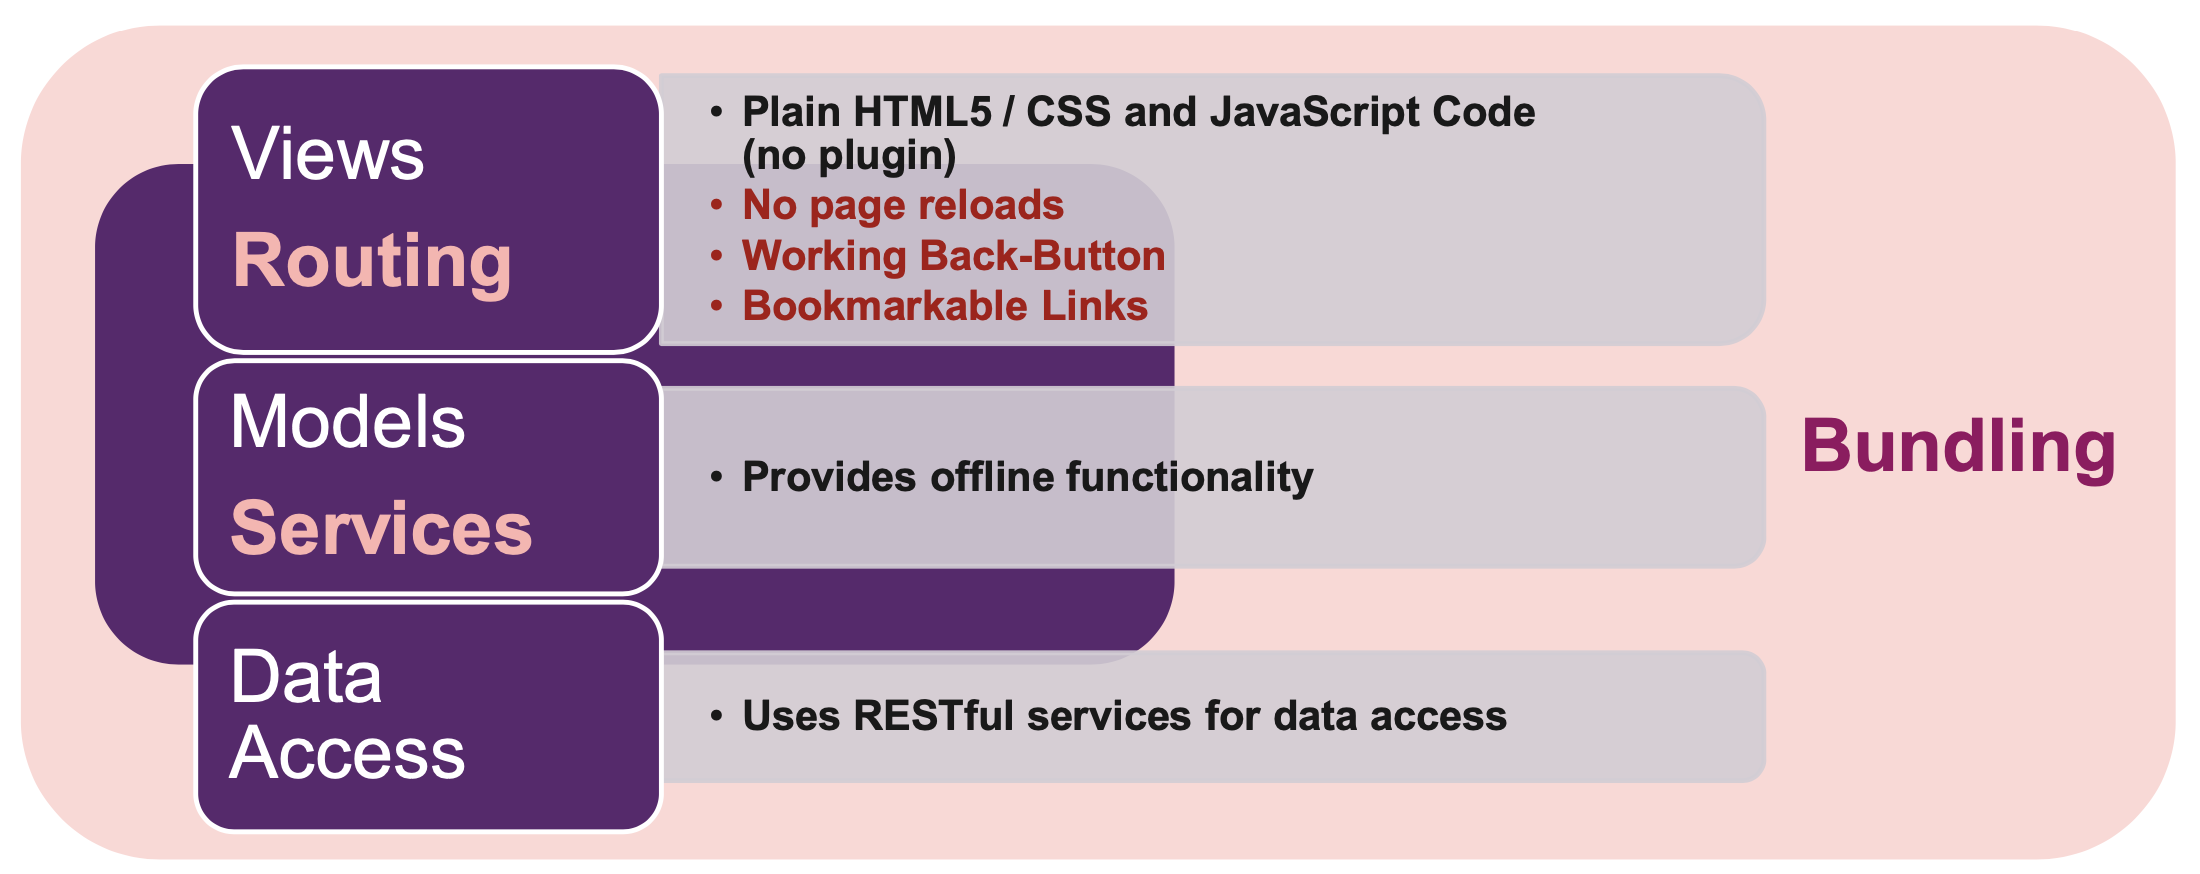
\includegraphics[width=\linewidth]{spa_logical_overview}

        \textbf{Bundeling}: Gesamter JavaScript-Code muss über tendenziell langsame Leitung zu Kunden, bundling und minifying reduziert Grösse, grosse SPAs brauchen vernünftiges Dependency Management, Module können auch On-Demand geladen werden, Bundler kommen und gehen (z.B. Webpack, Grunt, Rollup, esbuild)
        Webpack:

        \begin{itemize}
            \item Entry: Startpunkt wo Webpack mit Bundling beginnt und Dependencies findet.
            \item Output: Wo sollen die finalen Dateien hingeschrieben werden?
            \item Loaders: Transformiert Dateien in Module.
            \item Plugins: Können zusätzliche Funktionalitäten bieten (z.B. Asset Management)
            \item Mode: Aktivierung bestimmter Optimierungstechniken nach Bedarf.
        \end{itemize}

        \textbf{Routing}: Wird in SPAs komplett client-seitig gemacht, Browser "fakt" URL-Änderungen, Content muss für Zurück-Button persistiert werden.
        Früher gelöst mittels \#, heute mit \lstinline{window.history} / \lstinline{window.history.pushState}, verhindert das der Browser die URL wirklich lädt.
        Meistens gelöst über eine Routing-Tabelle, welche je nach verlangter Route eine andere Funktion aufruft.

        \textbf{Dependency Injection}: Reduziert Kopplung zwischen Konsument und Implementation, "Verträge" zwischen Klassen basieren auf Interfaces, erlaubt flexible Ersetzung einer konkreten Implementieren.


        \section{React}

        Eine Bibliothek, kein Framework!
        Umfasst nur das V aus MVC.
        \textbf{Prinzip von React}: Komplexe Probleme in kleinere Komponenten aufteilen.
        Verbessert Wiederverwendbarkeit, Erweiterbarkeit, Wartbarkeit, Testbarkeit, Aufgabenverteilung im Team.

        \textbf{JSX}: React-Komponenten sind Funktionen, welche HTML zurückgeben können (JSX).
        JSX kann an beliebigen Stellen verwendet werden, wenn Dateiendung stimmt.
        In eckigen Klammern stehen dann JavaScript-Expresssions.
        Einschränkung: React-Elemente müssen mit Grossbuchstaben starten, \lstinline{className} anstatt \lstinline{class} verwenden wegen gesperrter Keywords.
        Unterelement sind mittels \lstinline{props.children} zugänglich.
        \lstinline{props} als read-only behandeln!

        \begin{lstlisting}
        function Container(props) {
            return (
            <div className="container">
                {props.children}</div>
            )
        }

        function App() {
            return (
                <Container><HelloMessage name="OST"/></Container>
            )
        }
        \end{lstlisting}

        Styles werden als Objekt übergeben, muss Camel Case verwenden (\lstinline{min-height} wird zu \lstinline{minHeight}).
        Die JSX-Elemente werden zu \lstinline{React.createElement} umgewandelt, daher muss in jedem JSX-File React importiert werden, auch wenn es nicht aktiv verwendet wird.

        \begin{lstlisting}
        function Container(props) {
          return React.createElement("div",
            { className: "container" },
            props.children
          )
        }
        \end{lstlisting}

        React-Kompontenten konnten früher mittels Klasse definiert werden.
        Seit den Hooks aber nicht mehr nötig.

        \begin{lstlisting}
        class HelloMessage extends React.Component {
          render() {
            return <div>Hello {this.props.name}</div>
          }
        }
        \end{lstlisting}

        Anlegen einer neuen App: \lstinline{npx create-react-app hello-ost}.
        Konfiguration kommt dann aus einem NPM-Paket (Webpack, Babel, etc.).
        Kann mittels \lstinline{eject} entfernt werden.

        \textbf{Mount}: Komponenten müssen mittels Instruktion gemountet werden.
        Theoretisch mehrere Mounts pro Webseite möglich.

        \begin{lstlisting}
        import React from 'react';
        import ReactDOM from 'react-dom/client';
        import App from './App';

        const root = ReactDOM.createRoot(document.getElementById('root')); root.render(<App />);
        \end{lstlisting}

        \textbf{State}: Mittels \lstinline{useState} Hook.
        \lstinline{useState} müssen immer in derselben Reihenfolge erfolgen, somit if-Konditionen nicht möglich.
        State einer Komponente ist immer privat, kann aber als Props weitergegeben werden.
        Auch Event-Handler / Setter können als Props an Komponenten weiter gegeben werden.
        Zustand darf ausschliesslich mit Settern geändert werden.

        \begin{lstlisting}
        import { useState } from 'react';

        function Counter() {
          const [counter, setCounter] = useState(0);
          const increment = () => setCounter(counter + 1);
          return (
            <div>
              <p>{counter}</p>
              <button onClick={increment}>Increment Counter</button> </div>
          )
        }
        \end{lstlisting}

        \textbf{Reconciliation}: React-Komponenten werden als virtueller DOM gerendert, Wird der State geändert, erstellt React einen neuen virtuellen DOM, alter und neuer DOM werden verglichen, erst dann werden geänderte DOM-Knoten im Browser erstellt.

        \textbf{Formulare}: Event Handler bei den Inputs registrieren und Zustand ändern.

        \begin{lstlisting}
        <input value={username} type="text" onChange={e => setUsername(e.target.value)} />
        \end{lstlisting}

        Oder mittels \lstinline{onSubmit} auf dem Formular abfangen.

        \begin{lstlisting}
        function handleSubmit(event) {
            event.preventDefault();
            alert("Username: " + username + ", Password: " + password)
        }
        \end{lstlisting}

        \textbf{Styling}: Meistens mittels Widget-Library, z.B. Reactstrap, Material UI oder Semantic.

        \textbf{Lifecycles}: Klassenkomponenten haben eine Reihe an Lifecycle-Methoden wie \lstinline{componentDidMount} , \lstinline{shouldComponentUpdate(nextProps, nextState)} oder \lstinline{componentWillUnmount}.
        Mit Hooks vereinfacht mit \lstinline{useEffect}.
        \lstinline{useEffect} kann mit Promises verwendet werden.

        \begin{lstlisting}
        useEffect(() => {
          const timerID = setInterval(() => setDate(new Date()), 1000) // ausgefuehrt beim Mount
          return () => {
            clearInterval(timerID) // ausgefuehrt beim Unmount
          }
        }, []) // Arrays von Dependencies, kann genutzt werden, um Effekt auszuloesen, wenn sich Abhaengigkeit aendert
        \end{lstlisting}

        \textbf{Routing}: Mittels React Router (Kollektion von Navigationskomponenten für React, für Web und Native).
        Alle Router müssen Teil von \lstinline{<BrowserRouter>} sein.
        \lstinline[mathescape]!<Route path="/about" element ={<About/>} />!: Component About wird nur gerendert, wenn der path matcht.
        App-interne Links verwenden nicht <a> sondern <Link>. \lstinline[mathescape]!<Link to="/about">About</Link>!

        \textbf{Type-Checking}: Flow erweitert JavaScript um Typannotationen.
        Lieber Typescript für mehr Typsicherheit in React-Komponenten.
        Flow sind nur Annotations, können daher einfach ignoriert werden, Typescript ist eine ganze Programmiersprache.

        \textbf{React Context}: Daten immer als Props mitgeben ist mühsam, Zustand verteilt sich über gesamte Applikation, Calls sind auch verteilt.
        React Context ermöglicht es, Props für alle Unterkomponenten zur Verfügung zu stellen.

        \begin{lstlisting}
        const ThemeContext = React.createContext(themes.light);

        function App() {
          return (
            <ThemeContext.Provider
              value={themes.dark}>
              <Toolbar />
            </ThemeContext.Provider>
          );
        }

        function ThemedButton() {
          const theme = useContext(ThemeContext);
          return (
            <button style={{
              background: theme.background,
              color: theme.foreground
            }}>
              {" "}I am styled by theme context!{" "}
            </button>
          );
        }
        \end{lstlisting}

        \textbf{Redux}: Darstellung des States als Baum, Baum ist nicht veränderbar, Veränderungen am Baum führen zu einem neuen Baum, Verwaltung über Stores.

        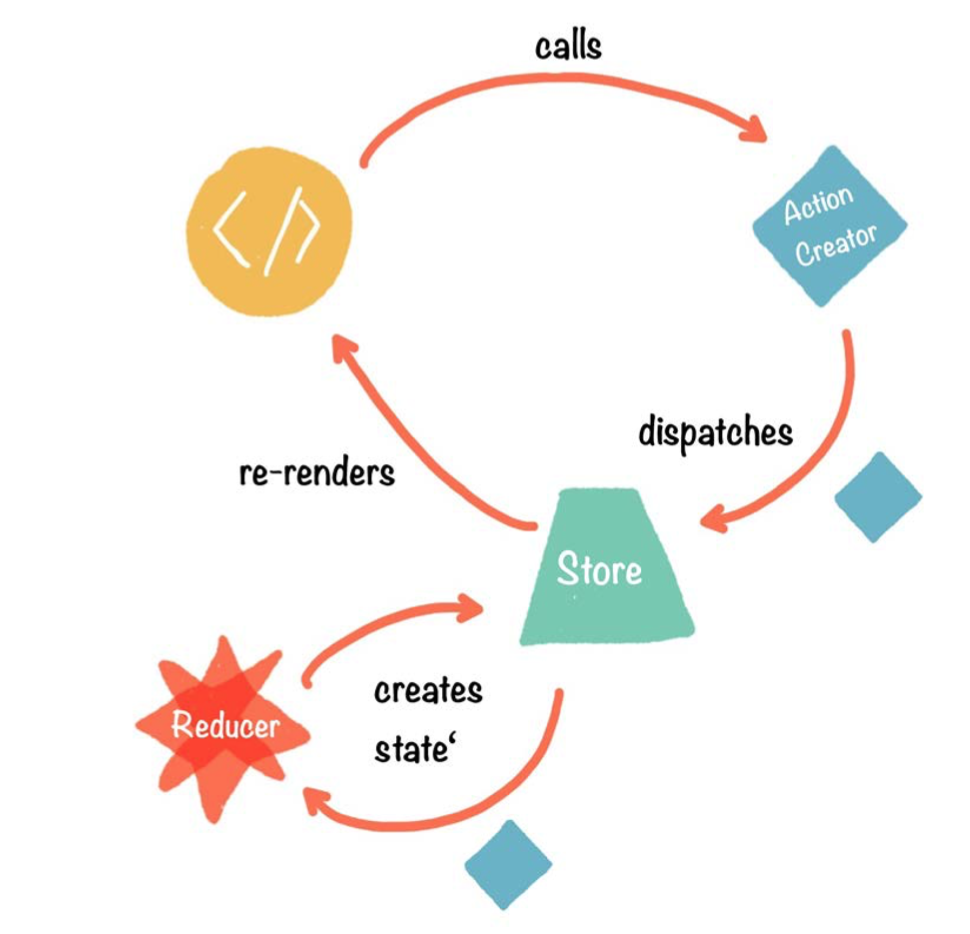
\includegraphics[width=\linewidth]{redux_data_flow}

        Eine Veränderung braucht eine Action (sehr simple Objekte wie \lstinline!{ type: 'TRANSFER', amount: 100 }!).
        Der Store braucht einen Reducer, um mit der Action den neuen Baum zu machen.
        Reducer sind pure Funktionen ohne Seiteneffekte.

        Soll / Muss in jeder React-Applikation Redux eingesetzt werden?
        Nein, wenn kaum Zustand existiert, der von mehreren Komponenten verwendet wird, lohnt sich der Redux-Overhead nicht.

        \begin{lstlisting}
        function balance(state = 0, action) {
          switch (action.type) {
            case 'TRANSFER':
              return (
                state + action.amount
              )
            default:
              return state
          }
        }
        \end{lstlisting}

        Mehrere Reducer bilden einen Root Reducer.
        Initialer State für die App ist ein leeres Objekt.

        \begin{lstlisting}
        function rootReducer(state = {}, action) {
          return {
            balance: balance(state.balance, action),
            transactions: transactions(state.transactions, action)
          }
        }

        // gleichwertig
        const rootReducer = combineReducers({
           balance,
           transactions
        })

        const store = createStore(rootReducer);
        \end{lstlisting}

        Über Änderungen am State kann man sich mittels Listener benachrichtigen lassen: \lstinline{store.subscribe(() => console.log(store.getState()));}

        \textbf{React und Redux}: Redux Toolkit verwenden.
        \lstinline{createSlice} erstellt neue Stateobjekte, Reduce-Funktionen und Aktionen.
        Action-Type im unteren Beispiel ist \lstinline{balance/transfer}.
        Mittels immer.js scheinbare, direkte Änderungen am State möglich.

        \begin{lstlisting}
        const balanceSlice = createSlice({
          name: "balance",
          initialState: { value: 0 },
          reducers: {
            transfer: (state, action) => {
              state.value += action.payload.amount;
            },
          },
        });
        export const { transfer } = balanceSlice.actions;
        \end{lstlisting}

        \lstinline{configureStore} initialisiert den Redux Store mit den angegeben Reducern.
        Enthält \lstinline{redux-thunk}.
        Redux Thunk erlaubt es uns, anstelle eines Objektes eine Funktion zu dispatchen.

        \begin{lstlisting}
        const store = configureStore({
          reducer: { balance: balanceReducer }
        });
        \end{lstlisting}

        Verfügbarkeit in React-Applikation mittels Provider.

        \begin{lstlisting}
        render(
          <Provider store={store}>
            <App />
          </Provider>,
          document.getElementById('root')
        )
        \end{lstlisting}

        \lstinline{useDispatch} wird für den Dispatch der Aktionen an den Store benutzt.
        \lstinline{useSelector} wird für die Abfrage des States benutzt.

        \begin{lstlisting}
        const dispatch = useDispatch()
        dispatch(transfer({ amount: 10 }))
        const balance = useSelector(state => state.balance.value);
        \end{lstlisting}

        Asynchrone Actions:

        \begin{lstlisting}
        // First, create the thunk
        export const transferAsync = createAsyncThunk(
          "balance/transferApiRequest",
          async (amount) => {
            const response = await api.transfer(amount);
            return response.data;
          }
        );

        const balanceSlice = createSlice({
          initialState: { value: 0, status: "idle" },
          extraReducers: (builder) => {
            builder
              .addCase(transferAsync.pending, (state) => {
                state.status = "loading";
              })
              .addCase(transferAsync.fulfilled, (state, action) => {
                state.status = "idle";
                state.value += action.payload.amount;
              });
          },
        });
        \end{lstlisting}

        \textbf{JHipster}: Fullstack App-Generator mit Angular, React-Redux oder Vue, Spring Boot, Maven/Gradle, NPM, Postgres, MongoDB, Elasticsearch, Cassandra, Kafka etc.
        Bieten eigene DSL für Entities und Relationen.

        \textbf{Testing}: Jest offizielle Lösung von Facebook, kommt mit \lstinline{create-react-app} mit.
        Die React Testing Library baut auf der DOM Testing Library auf und fügt APIs für die Arbeit mit React-Komponenten hinzu.
        JHipster generiert End-to-End-Tests mit Cypress.

        \begin{lstlisting}
        import { render, screen } from '@testing-library/react'
        import userEvent from '@testing-library/user-event'

        test('loads and displays greeting', async () => {
          // ARRANGE
          render(<Fetch url="/greeting" />)

          // ACT
          await userEvent.click(screen.getByText('Load Greeting'))
          await screen.findByRole('heading')

          // ASSERT
          expect(screen.getByRole('heading')).toHaveTextContent('hello there')
          expect(screen.getByRole('button')).toBeDisabled()
        })
        \end{lstlisting}


        \section{Angular}

        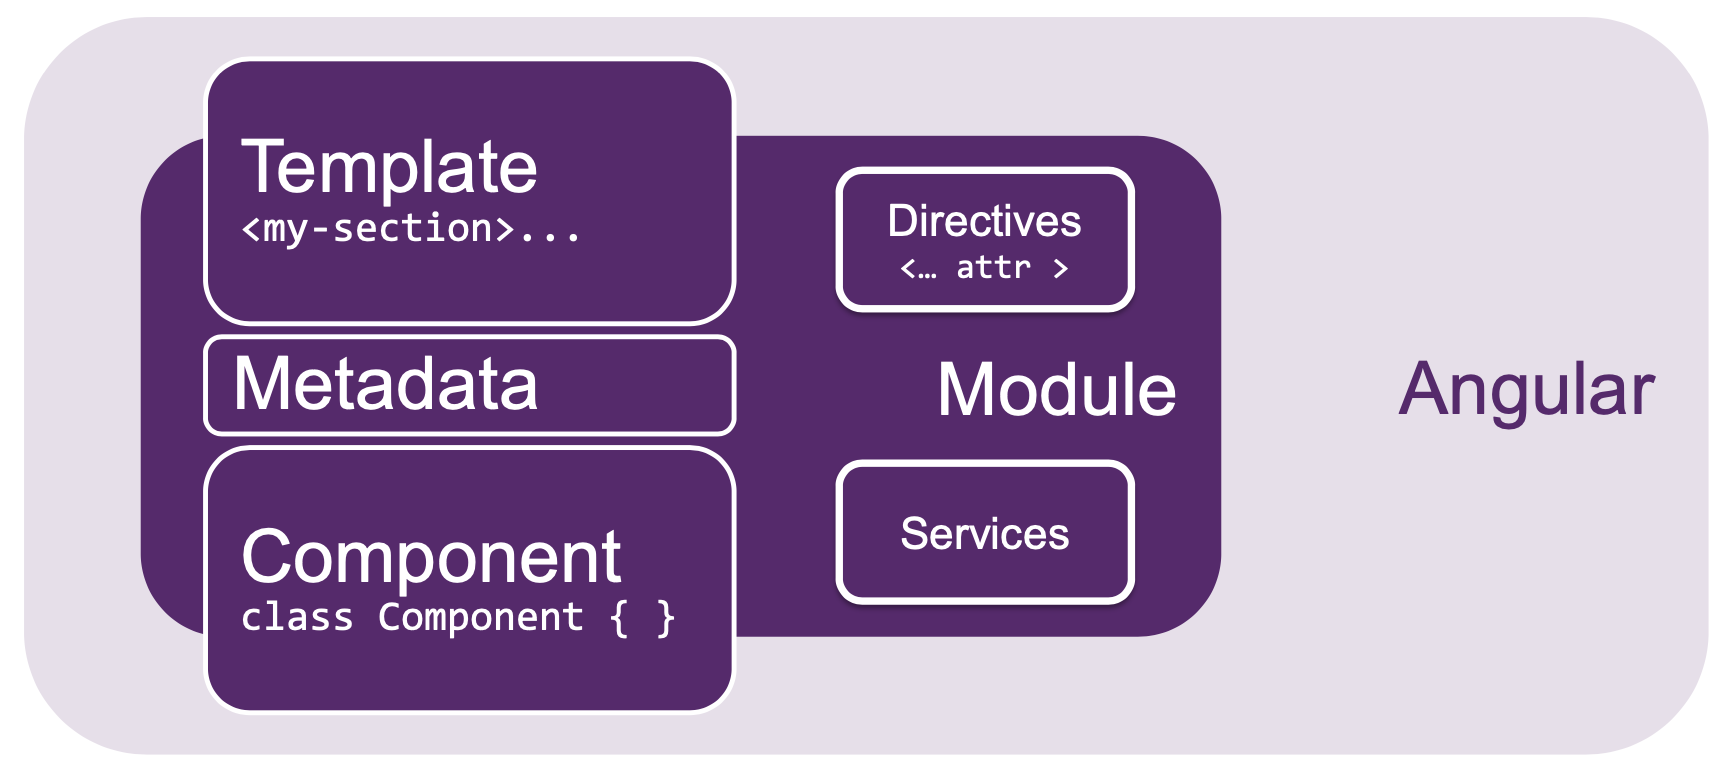
\includegraphics[width=\linewidth]{base_angular}

        TypeScript-basiert, mit Dependency Injection, 2-Way-Bindings, klar strukturiert.
        Sollte verwendet werden für lang lebende und komplexe Applikationen.
        Historie: Modernes Angular seit v2, v1 wird AngularJS genannt, keine Gemeinsamkeiten.
        v3 ausgelassen, um Paketnamen zu harmonisieren.
        \lstinline{npx ng new my-app} legt neue Applikation an (Paket lokal installieren mit \lstinline{npm install @angular/cli})

        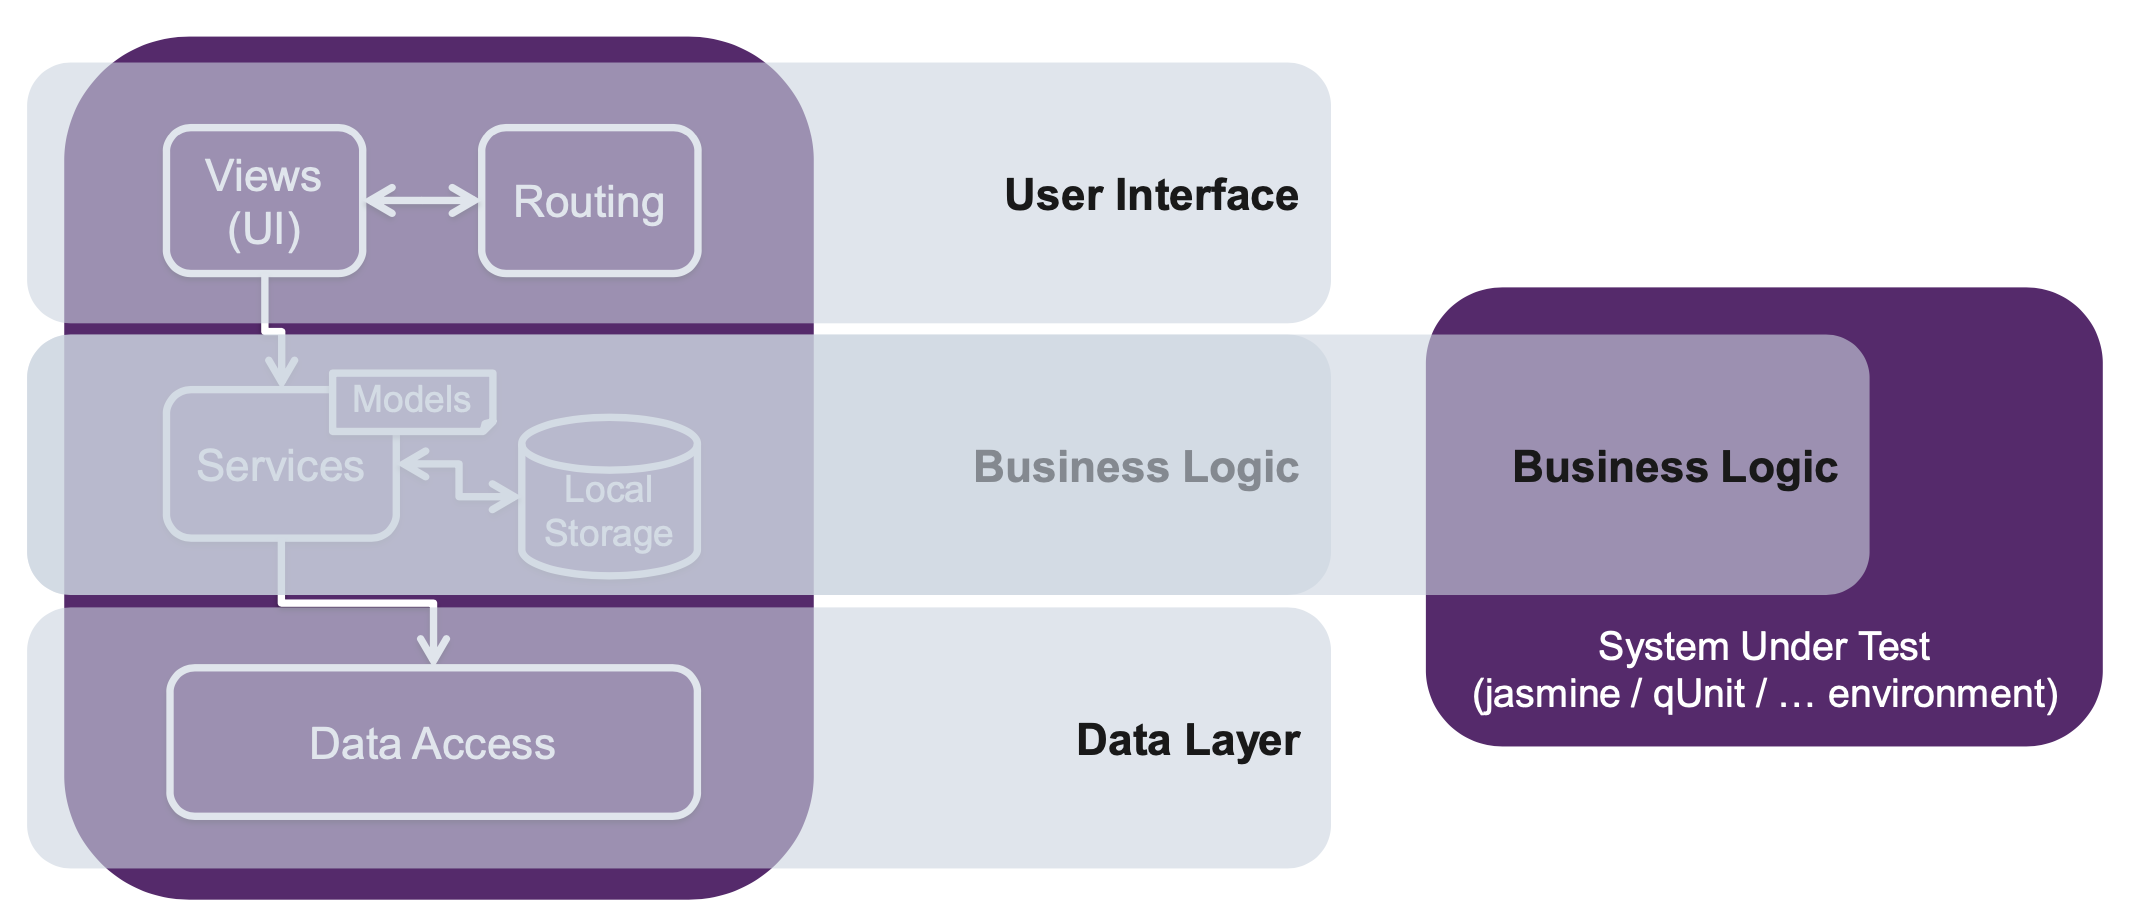
\includegraphics[width=\linewidth]{angular_logical_layers}

        \textbf{Dependency Injection}: Registration beim Container, Request, Resolve durch Container, Fullfill (TypeScript module/s).
        \textbf{ngModules}: Ein zusammenhängender Codeblock, der eng miteinander verbundenen Fähigkeiten gewidmet ist (TypeScript class).
        Jede App hat mindestens ein Modul, das Root-Modul.
        Exportieren Features wie Services oder Direktive für andere Module.
        ngModule-Deklaration selbst wird in ein TypeScript-Modul eingefügt (meistens über \lstinline{index.ts}).

        \begin{lstlisting}
        @NgModule({
            exports: [] // The subset of declarations that should be visible and usable in the component templates of other modules.
            imports: [CommonModule], // Specifies the modules which exports/providers should be imported into this module.
            declarations: [], // The view classes that belong to this module (components, directives and pipes).
            providers: [], // Creators of services that this module contributes to the global collection of services (Dependency Injection Container); they become accessible in all parts of the app.
            bootstrap: [] // The main application view, called the root component. Only the root module should set this property.
        })

        export class CoreModule { }
        \end{lstlisting}

        \textbf{Directives}: Enthält Anweisungen zur Transformation des DOM (TypeScript class).
        \textbf{Components}: Eine Komponente ist eine Richtlinie mit einer Vorlage; sie steuert einen Abschnitt der Ansicht (HTML File / (S)CSS / \ldots).
        Basiert auf MVC oder MVVM.
        Eine Komponente sollte so klein und zusammenhängend wie möglich implementiert werden, um die Testbarkeit / Wartbarkeit / Wiederverwendbarkeit zu unterstützen.
        \textbf{Metadata}: Metadaten beschreiben eine Klasse und sagen Angular, wie sie zu verarbeiten ist (TypeScript decorator).
        \textbf{Services}: Bietet Logik für jeden Wert, jede Funktion oder jedes Merkmal, das Ihre Anwendung benötigt (TypeScript class).
    \end{multicols}
\end{document}
